% !TeX document-id = {2cd55586-af93-4ea8-9988-33759386929e}
% !TEX program = pdflatex
% !BIB program = biber
\documentclass[11pt,
	a4paper,
	ngerman,
	bibliography=totoc,
	captions=tableheading,
	headings=normal,
	parskip=half*,
	chapterentrydots=true,
	numbers=noenddot
	]{scrreprt}

% load packages
%!TEX root = main.tex
\usepackage[T1]{fontenc}
\usepackage[utf8]{inputenc}
\usepackage[ngerman]{babel}
%\usepackage[scaled=1]{uarial} % set default font to arial
\renewcommand{\familydefault}{\sfdefault}
\usepackage{bm} 
\usepackage{multirow}
\usepackage{float}

% enable hyperlinks in pdf documennt
\usepackage[hidelinks]{hyperref}
%\usepackage[colorinlistoftodos]{todonotes}\reversemarginpar

% Import the stuff for the glossary
\usepackage[numberedsection,nonumberlist,acronym,toc,nopostdot,nomain]{glossaries}
\newglossary[slg]{symbolslist}{syi}{syg}{Formelzeichen und Indizes} % create add. symbolslist
\makeglossaries
\setacronymstyle{long-short}
\loadglsentries[acronyms]{acronym_entries.tex}
\loadglsentries[symbolslist]{symbol_entries.tex}

%% the following commands are needed for some matlab2tikz features
%\usetikzlibrary{plotmarks}
%\usetikzlibrary{arrows.meta}

\usepackage{graphicx}
\usepackage{tkz-euclide}
\usetkzobj{all}
\usepackage{pgfplots}
\usepackage{tikzscale}
\pgfplotsset{
    every tick label/.append style = {/pgf/number format/assume math mode=true,font=\sffamily},
}
\pgfplotsset{max space between ticks=50}
\pgfplotsset{compat=newest}


\usepackage{grffile}
\usepackage{amsmath}
\usepackage{listings}
\usepackage{rotating}
\usepackage{cleveref}
%\crefname{equation}{eq.}{eqs.}
%\Crefname{equation}{Eq.}{Eqs.}
\crefformat{equation}{Gl.~#2#1#3}
\Crefformat{equation}{Gl.~#2#1#3}
%\crefformat{subfigure}{Fig.~#2(#1)#3}
\crefname{table}{Abb.}{Tab.}
\crefname{figure}{Abb.}{Abb.}
\Crefname{table}{Tab.}{Tab.}
\crefname{chapter}{Kap.}{Kap.}
\Crefname{chapter}{Kap.}{Kap.}
\crefname{appendix}{Anhang}{}
\crefname{section}{Kap.}{Kap.}
\Crefname{section}{Kap.}{Kap.}
\crefname{subsection}{Kap.}{Kap.}
\Crefname{subsection}{Kap.}{Kap.}
\crefname{subsubsection}{Kap.}{Kap.}
\Crefname{subsubsection}{Kap.}{Kap.}

\usepackage{array}
\usepackage{booktabs}
\usepackage{color}
\usepackage{tensor}
\usepackage{pdfpages}
\usepackage{bm}
\usepackage[section]{placeins}

% set page margins etc.
\usepackage[
	headheight=1.25cm,
	headsep=1.25cm,
	left=3.0cm,
	right=2.0cm,
	top=3.0cm,
	bottom=2.5cm]{geometry}
	
\usepackage[labelformat=simple]{subcaption}
\usepackage[onehalfspacing]{setspace}
\AtBeginEnvironment{tabular}{\onehalfspacing}

\usepackage{amsmath}
\usepackage{amssymb}
\usepackage{siunitx}
\usepackage{tabto}
\usepackage{pbox}

%%%%%%%%%%%%%%%%%%%%%%%%%
% IKA - format	        %
%%%%%%%%%%%%%%%%%%%%%%%%%

%% labelin
%\newcommand{\reffig}[1]{Fig.~\ref{#1}}
%\newcommand{\refsec}[1]{Chapter~\ref{#1}}
%\newcommand{\refapp}[1]{Appendix~\ref{#1}}
%\newcommand{\refeq}[1]{Eq.~\ref{#1}}

% Anpassung der Gleichungsbeschriftung an das IKA-Layout, e.g. "Gl. 1-1"
\makeatletter
	\def\@eqnnum{{\normalfont \normalcolor Gl.\quad \theequation}}
	\def\tagform@#1{\maketag@@@{Gl.\quad\ignorespaces#1\unskip\@@italiccorr}}
\makeatother

% Anpassung der Tabellen- und Bildbeschriftung an das IKA-Layout, e.g. "Abb. 1-1:	" (Teil 2)
\usepackage[titles]{tocloft}
\renewcaptionname{ngerman}{\figurename}{Abb.}
\renewcommand{\cftfigpresnum}{Abb. }
\renewcommand{\cftfigaftersnum}{:}
\settowidth{\cftfignumwidth}{Abb. 10\quad}
\renewcaptionname{ngerman}{\tablename}{Tab.}
\renewcommand{\thefigure}{{\thechapter-\arabic{figure}}}
\renewcommand{\thetable}{{\thechapter-\arabic{figure}}}
\renewcommand{\theequation}{{\thechapter-\arabic{equation}}}

% Durchgehende Nummerierung f�r Abbildungen und Tabellen: IKA fordert Tabllen mit Abb-Caption: Abb. X-Y
\makeatletter
\let\c@table\c@figure
\makeatother


% Anpassung der Beschriftungen
\usepackage[
	style=base,
	font=onehalfspacing,
	format=hang,
	margin=0cm,
	singlelinecheck=false,
	skip=6pt
	]{caption}

% Anpassung der Abs�tze vor und nach einer figure Umgebung
\setlength{\intextsep}{12pt}

\renewcommand{\thesubfigure}{(\roman{subfigure})}


% Kopf- und Fu�zeile
%%%%%%%%%%%%%%%%%%%%%%
%\usepackage[
%	headsepline=0.75pt,
%	plainheadsepline=true,
%	footsepline=false,
%	plainfootsepline
%	]{scrlayer-scrpage} % F�r die Kopf- und Fu�zeile inkl. Trennlinie und Titel gro� geschrieben
%

%
%\ihead*[\thechapter \tabto{1cm}{\leftmark}]{\thechapter \tabto{1cm}{\leftmark}}
%\cohead*[]{}
%\rohead*[\thepage]{\thepage}
%\ifoot*[]{}
%\cofoot*[]{}
%\rofoot*[]{}
\usepackage{fancyhdr}

\pagestyle{fancy}
\renewcommand{\chaptermark}[1]{\markboth{#1}{}}

\fancypagestyle{ika}{%
    \fancyhf{}
    \lhead{\thechapter \tabto{1cm} \leftmark}
    \rhead{\thepage}
    \fancyfoot[]{}
}
\fancypagestyle{plain}{%
    \fancyhf{}
    \lhead{\leftmark}
    \rhead{\thepage}
    \fancyfoot[]{}
}
\fancypagestyle{apx}{%
    \fancyhf{}
    \lhead{Appendix - \leftmark}
    \rhead{\thepage}
    \fancyfoot[]{}
}
\renewcommand{\headrulewidth}{0.75pt}


% XML Listing
\definecolor{gray}{rgb}{0.4,0.4,0.4}
\definecolor{darkblue}{rgb}{0.0,0.0,0.6}
\definecolor{cyan}{rgb}{0.0,0.6,0.6}

\lstset{
    basicstyle=\ttfamily,
    columns=fullflexible,
    frame = single, 
    numbers = left,
    showstringspaces=false,
    commentstyle=\color{gray}\upshape
}

\lstdefinelanguage{XML}
{
    morestring=[b]",
    morestring=[s]{>}{<},
    morecomment=[s]{<?}{?>},
    stringstyle=\color{black},
    identifierstyle=\color{darkblue},
    keywordstyle=\color{cyan},
    morekeywords={}% list your attributes here
}
\pgfkeys{/pgf/number format/.cd,1000 sep={}}
%%%%%%%%%%%%%%%%%%%%%%%%%%%%%%%%%%
% Formatierung der �berschriften
%%%%%%%%%%%%%%%%%%%%%%%%%%%%%%%%%%

% Kapitel�berschrift
\RedeclareSectionCommands[
  afterskip=4pt,
  beforeskip=4pt
]{chapter}

% Unterkapitel
\RedeclareSectionCommands[
  afterskip=4pt,
  beforeskip=4pt
]{section}

\RedeclareSectionCommands[
  afterskip=4pt,
  beforeskip=4pt
]{subsection}

% Unterkapitel
\RedeclareSectionCommands[
  afterskip=4pt,
  beforeskip=4pt
]{subsubsection}

\RedeclareSectionCommands[
  tocindent=0.3cm
]{section}

\RedeclareSectionCommands[
  tocindent=0.6cm
]{subsection}

\RedeclareSectionCommands[
  tocindent=0.9cm
]{subsubsection}

%\RedeclareSectionCommands[
%  tocbeforeskip=5pt
%]{section,subsection,subsubsection}

% Tabstopp f�r �berschriften auf 1cm setzen
\renewcommand*{\chapterformat}{%
	\makebox[1cm][l]{\chapappifchapterprefix{\nobreakspace}\thechapter
	\IfUsePrefixLine{}}}
\renewcommand*{\sectionformat}{%
	\makebox[2cm][l]{\thesection}}
\renewcommand*{\subsectionformat}{%
	\makebox[2cm][l]{\thesubsection}}
\renewcommand*{\subsubsectionformat}{%
	\makebox[2cm][l]{\thesubsubsection}}

% Schriftarten
\setkomafont{chapter}{\normalfont\bfseries}
\setkomafont{section}{\normalfont\bfseries}
\setkomafont{subsection}{\normalfont\bfseries}
\setkomafont{subsubsection}{\normalfont\bfseries}
\setkomafont{pagehead}{\normalfont}
\setkomafont{chapterentry}{\normalfont}


% RWTH Farbdefinitionen
\definecolor{blueRWTH}{cmyk}{1.0,0.5,0,0}
\definecolor{blueLightRWTH}{cmyk}{0.75,0.38,0,0}
\definecolor{blueLighterRWTH}{cmyk}{0.45,0.14,0,0}

\definecolor{greenRWTH}{cmyk}{0.7,0.0,1.0,0}
\definecolor{greenLightRWTH}{cmyk}{0.525,0,0.75,0}
\definecolor{greenLighterRWTH}{cmyk}{0.35,0,0.5,0}

\definecolor{orangeRWTH}{cmyk}{0,0.4,1.0,0}
\definecolor{orangeLightRWTH}{cmyk}{0,0.3,0.75,0}
\definecolor{orangeLighterRWTH}{cmyk}{0,0.2,0.5,0}

\definecolor{redRWTH}{cmyk}{0.15,1,1,0}
\definecolor{redLightRWTH}{cmyk}{0.1125,0.75,0.75,0}
\definecolor{redLighterRWTH}{cmyk}{0.075,0.5,0.5,0}
\definecolor{rwthLight}{cmyk}{0.0,0.0,0.0,0.5}

% no pagebreak
\usepackage{etoolbox}
\makeatletter
\patchcmd{\scr@startchapter}{\if@openright\cleardoublepage\else\clearpage\fi}{}{}{}
\makeatother

% literature and biber settings
%%!TEX root = main.tex
%%%%%%%%%%%%%%%%%%%%%%%%%%%%%%%%%%%%%%%%%%%%%%%%%%%%%%%%%%
%
% Literaturverzeichnis basierend auf:
% Biblatex mit Biber als Backend
%
%%%%%%%%%%%%%%%%%%%%%%%%%%%%%%%%%%%%%%%%%%%%%%%%%%%%%%%%%%
\usepackage[babel,german=guillemets]{csquotes}

\usepackage[
	backend=biber,
	style=alphabetic,
	url=false, 
    doi=false,
    isbn=false,
    maxbibnames=99,
    giveninits=true,
    maxalphanames=1
	]{biblatex}

\addbibresource{literature/literature_masterthesis.bib}


\renewcommand*{\mkbibnamefamily}[1]{\MakeUppercase{#1}}	% UpperCase für Namen
\renewcommand*{\newunitpunct}{\addcomma\space}   		% Komma statt Punkt
\renewcommand*{\finentrypunct}{}                        % kein Punkt am Ende der Einträge
\DeclareFieldFormat[article, book, inbook, inproceedings, misc, techreport, phdthesis]{citetitle}{#1}
\DeclareFieldFormat[article, book, inbook, inproceedings, misc, techreport, phdthesis]{title}{#1}

\renewcommand*{\labelnamepunct}{\newline}				% Zeilenumbruch statt Komma hinter Autoren
\renewcommand*{\labelalphaothers}{}						% "+" bei mehreren Autoren entfernen
\renewbibmacro{in:}{}									% "in:" Zusatz bei Artikel in Journaleinträgen entfernen
\renewcommand*{\bibfont}{}
\renewcommand*{\finalnamedelim}{\addsemicolon\space} %semicolon zwischen letztem und vorletztem Autor
\renewcommand*{\multinamedelim}{\addsemicolon\space} %semicolon zwischen Autoren

% Formatierung der Zitierungslabels
\DeclareLabelalphaTemplate{
  \labelelement{
    \field[uppercase,final]{shorthand}
    \field[uppercase]{label}
    \field[uppercase,strwidth=3,strside=left,ifnames=1]{labelname}
    \field[uppercase,strwidth=1,strside=left]{labelname}
  }
  \labelelement{
    \field[strwidth=2,strside=right]{year}
  }
}

% et al. statt u.a. 
\DefineBibliographyStrings{german}{
   andothers = {{et al\adddot}},            
}

%\pagestyle{scrheadings}
\setcounter{secnumdepth}{4} % sections numbered until 4th layer
\setcounter{tocdepth}{4} % include headings into toc until 4th layer
\begin{document}

%\listoftodos \newpage
%
\includepdf{CoverSheet.pdf}
\title{CES-Seminararbeit  \\ Implementierung und Absicherung eines Tools zur Generierung von virtuellen Strassen und Kreuzungen im openDRIVE Format}
\author{Christian Geller \\  Mat.-Nr. 344934 \\ Daniel Becker, Institut für Kraftfahrzeuge, RWTH Aachen}
\maketitle
%\newpage

% uncomment for empty page
\thispagestyle{empty}
%\mbox{}
%\newpage
\pagenumbering{arabic}
\pagestyle{plain}
\setcounter{page}{3}
\renewcommand{\contentsname}{Inhalt}
\tableofcontents
\newpage
%\pagestyle{ika}
%!TEX root = ../main.tex
\chapter{Einleitung}
%\thispagestyle{ika}

In der Automobilindustrie geht der Trend in den vergangenen Jahren verstärkt zu der Entwicklung und Realisierung von autonomen Fahrfunktionen. Um diese automatisierten Fahrmanöver validieren zu können werden Simulationen als Abbild der Realität herangezogen. Ausgangspunkt jeder Simulation ist eine vorhandene Streckenbeschreibung, die sich grundsätzlich zerlegen lässt in die Strasse als solche, die Verkehrsinfrastruktur wie Beschilderungen oder Ampelanlagen und temporären Veränderungen wie zum Beispiel Baustellen. Zum einen können solche Strecken anhand der Realität erzeugt werden, was jedoch einen hohen detaillierungsgrad vorrausetzt und sich als sehr aufwendig gestaltet. Eine weitere Möglichkeit zur erzeugung von Strecken ist ein logisch, varierbarer Ansatz der als Grundlage für diese Seminararbeit herangezogen wird. Es gilt hierbei nicht die Realität sondern Vorschriften und Grenzen einzuhalten und durch einfache und parametrisierte Angaben ein komplexes und vorallem valides Streckennetz generieren zu können.

Die Grundidee hierbei ist die Implementierung eines Tools mit Hilfe dessen der Benutzer ein vereinfachtes Eingabeformat füllt und als Resultat ein komplexes aber in sich valides Streckennetz erhält. Das Eingabeformat wurde als solches im Rahmen einer Masterarbeit klar definiert und ausgearbeitet. Die Hauptaufgabe dieser Seminararbeit besteht nun also in der Validierung und Absicherung des vorhanden Formates und einem Übersetzungstool dass die abstrakte Strecke in einem industriell gängigem Format liefert.

\chapter{OpenDrive Standard}
OpenDrive ist ein Format zur Darstellung von logischen Strassennetzwerken, welches seit 2006 existiert und mittlerweile als Standard für Fahrzeugsimulationen angesehen werden kann. Das Format enthält nicht nur Strassen und Fahrbahninformationen sondern auch komplexere Beschilderung, Fahrbahnmarkierungen und sogar Ampelsignale. Definiert wird die openDrive Datenstruktur im XML-Format in welcher grundsätzlich zwischen Strassen ('roads') und Kreuzungen ('junctions') unterschieden wird. Die logische Beschreibung der Strasse erfolgt anhand von einer analytischen Beschreibung, bestehend aus Geraden, Kreisbögen und Spiralen. Zudem kann die laterale Position und Ausrichtung sowie ihr Höhenprofil definiert werden. Die Geometrie einer Strasse wird immer über die Referenzlinie definiert, hinzugefügt werden dann einzelne Fahrbahnen ('lanes') mit unterschiedlicher Markierung, Breite, Beschafftenheit etc. An komplexen Kreuzungen werden die Fahrbahnverbindungen, welche ebenfalls als eigene Strasse im openDrive Format definiert sind über 'junctions' miteinander verbunden. Zudem lassen sich unbegrenzt Objekte definieren. Dies sichert eine eindeutige und korrekte Beschreibung der gewünschten Strecke, macht das XML-Format allerdings auch sehr komplex.  

\chapter{Annahmen und Vereinfachungen des ika Konzepts}
Wie im vorherigen Abschnitt gezeigt ist das openDrive Format zwar eindeutig und lässt quasi jede Art von Beschreibung der Strecke zu, allerdings ist die Generierung oder Befüllung des Formats sehr aufwendig und von Hand kaum zu realisieren. Deshalb existieren Tools mit denen man grafisch eine Strecke im geannten openDrive Format erzeugen kann. Um die Realtität abbilden möglichst gut abbilden zu können reicht dies zwar aus, alledings ist die varierbarkeit von Strecken ein grosser Vorteil bei der Simulation von Fahrmanövern zur Absicherung. So können mit wenigen Parameteränderungen beliebig viele, voneinander unterschiedliche aber valide Strecken generiert werden. Daher bedarf es ein Tool dass anhand eines einfachen, benutzerfreundlichen Eingangsformat das komplexe, detaillreiche openDrive Format generiert.

Im Unterschied zum openDrive Format werden von Nutzer nicht alle Strassen und Fahrbahnsegmente einzeln angegeben, sondern jede Kreuzung oder Verbindungsstrasse zunächst einzeln und unabhängig in einem eigenen Koordinatensystem definiert. Vorgegben durch den Nutzer werden nur die Geometrien der Haupt und Nebenstrassen. Am Beispiel einer Kreuzung werden diese dann benutzt um im Kreuzungsbereich zusätzlich und automatisiert Verbindungsstrassen zu generieren. Dazu wird lediglich der Kreuzungsschnittpunkt und der Winkel zwischen den zwei aufeinandertreffenden Strassen definiert. 

Die einzlenen Kreuzungssegmente werden in einem späteren Schritt dann aneinandergefügt. Der Nutzer spezifiziert dafür lediglich zwei Strassenpunkte auf den beiden Segmenten die übereinstimmen sollen. Mithilfe des Strassenwinkels und der Position ist die Lage dementsprechend eindeutig definiert. Das Koordinatensystem des einen Segments kann dementsprechend transformiert werden, sodass über eine einfache Beschreibung mehrere Kreuzungs oder Strassensegmente miteinander verbunden werden.

Um ein Strassennetzwerk schliessen zu können bedarf es einer sehr genauen konstuktion des letzten Segmentes, welches sich in einem überbestimmten Problem wiederspiegelt. Deshalb wird zum Schliessen eines Netzwerks eine separate Funktion entwickelt, die zwei Punkte unter entsprechendem Winkel miteinander verbindet.

Für den Nutzer sind also nur vereinfachte Angaben wie Krezungstyp, Strassengeometrie, Schnittwinkel oder Fahrbahnanzahl gefragt. Die Aufgabe des Tools ist nun die übersetzung in ein detaillreiches Strassennetzwerk im gängigen openDrive-Format.

\chapter{Umsetzung und Implementierung des Tools}
\section{Ein - und Ausgabeformat}
Die Definition im vereinfachten Eingabeformat geschieht ebenfalls wie die Darstellung des openDrive Formats im XML Format. Dies erlaubt eine Übersichtliche defintion der Datenstruktur mit Hilfe von 'Attributen' und 'Elementen'. Das Tool zur Generierung des openDrive-Formats wird in c++ geschrieben sodass eine kompatible Bibliothek zum parsen und schreiben der XML Dateien verwendet wird. Die Bibliothek 'pugi_xml' ermöglicht das einlesen der Eingabedatei und speichert die XML Struktur ähnlich einer Baumstruktur zur Laufzeit ab. Dies ermöglicht eine effiziente und übersichtliche Verwendung des Eingabeformats. Ebenso wird eine solche XML Stuktur zur Laufzeit des Tools erzeugt, die dann mit den openDrive Dateien gefüllt werden kann. 

Ein weiterer Vorteil bei der Benutzung von XML Datenstrukturen ist die Möglichkeit von XML Schemata (XSD). Eine .xsd Datei beschreibt die Struktur eines XML Dokumentes. So kann das Vorkommen von Attributen und Elementen eingeschränkt werden. So besteht die Möglichkeit die Anzahl von Elementen einzuschränken, die Anordnung von Elementen innerhalb des XML Dokuments vorzuschreiben oder Attribute nur optional vorzuschreiben. So wurde im Rahmen der Seminararbeit ein XML-Schema Dokument zur absicherung von falschen Benutzereingaben erstellt. Der gängige Standard openDrive besitzt ebenfalls eine solche Schemadatei, sodass sowohl Eingabe als auch Ausgabedokument mit Hilfe eines XML/XSD Validierungstools abgesichtert werden können.
 
\section{Implementierung}

\chapter{Beispiele und Tests}
\section{T-Kreuzung}
\section{X-Kruzung}
\section{Kreisverkehr}

\chapter{Ausblick}



%%!TEX root = ../main.tex
\chapter{Grundlagen und Stand der Technik}
\thispagestyle{ika}
\gls{ros} \gls{symb:ay}
\begin{figure}[H]
	\flushleft
	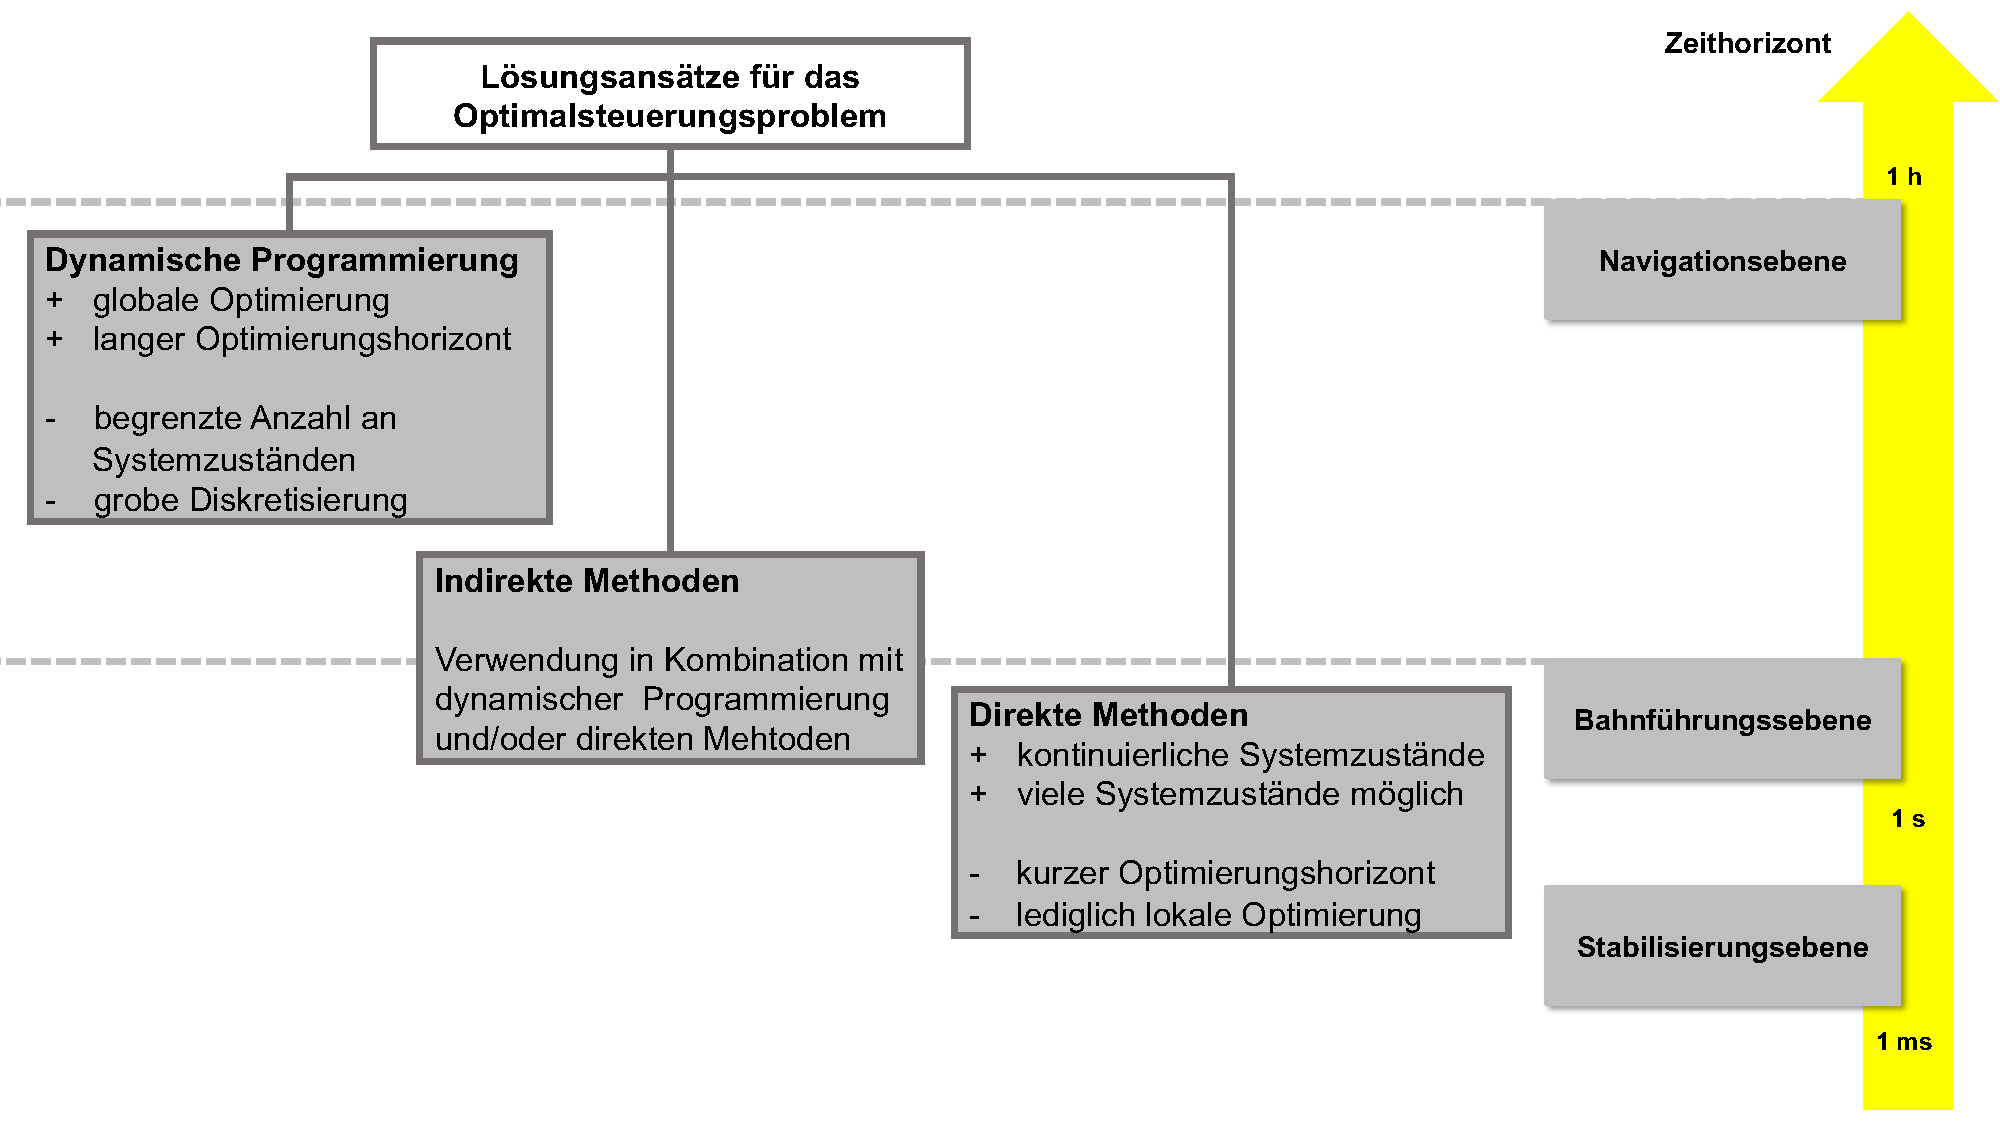
\includegraphics[width=0.95\textwidth]{content/fig/2_SdT/Einordnung_Planungsalgorithmen.pdf}
	\caption{Einordnung der Lösungsverfahren des Optimalsteuerungsproblems in das drei Ebenen Modell \cite{Donges.1982,Werling.2017}}
	\label{fig:EinordnungPlanungsalgorithmen}
\end{figure}
%%!TEX root = ../main.tex
\chapter{Forschungsvorhaben und Zielsetzung}
\label{kap:Forschungsvorhaben}
\thispagestyle{ika}

%%!TEX root = ../main.tex
\chapter{Umsetzung}
\label{kap:Umsetzung}
\thispagestyle{ika}

%%!TEX root = ../main.tex
\chapter{Ergebnisse und Bewertung}
\label{kap:Ergebnisse}
\thispagestyle{ika}
%%!TEX root = ../main.tex
\chapter{Zusammenfassung und Ausblick}
\label{kap:Zsmf}
\thispagestyle{ika}


\setlength\LTleft{-6pt}
\setlength\LTright{0pt}
%\printglossary[type=symbolslist,style=long,title=Formelzeichen und Indizes,toctitle=Formelzeichen und Indizes]
%\printglossary[type=acronym,style=long,title=Abkürzungen,toctitle=Abkürzungen]

%\newpage
%\pagestyle{plain}
%\listoffigures
%\addcontentsline{toc}{chapter}{\listfigurename}

\newpage
\pagestyle{plain}
\printbibliography[
	heading=bibnumbered,
	title=Literaturverzeichnis
]
\newpage
\pagestyle{apx}
%!TEX root = ../main.tex
\chapter{Anhang}
\label{kap:Anhang}


\end{document}